
\begin{enumerate}[label=\thesection.\arabic*.,ref=\thesection.\theenumi]
\numberwithin{equation}{enumi}
%
\item
\label{ch2_constraint}
Modify the code in problem \ref{convex_code} to find a graphical solution for minimising
\begin{align}
f\brak{\mbf{x}} 
%= (x_1-8)^2 + (x_2-6)^2
\end{align}
with constraint
\begin{align}
%\label{convex-constraint}
g\brak{\mbf{x}} \geq 0
%= x_1 + x_2 - 9 
\end{align}

%\solution 
%This problem reduces to finding the radius of the smallest circle in the shaded area in Fig. \ref{fig.2.4} .  It is clear that this radius is 0.
%%	
%\begin{lstlisting}
%wget https://raw.githubusercontent.com/gadepall/optimization/master/manual/codes/2.4.py
%\end{lstlisting}
%
%
%\begin{figure}[!ht]
%\centering
%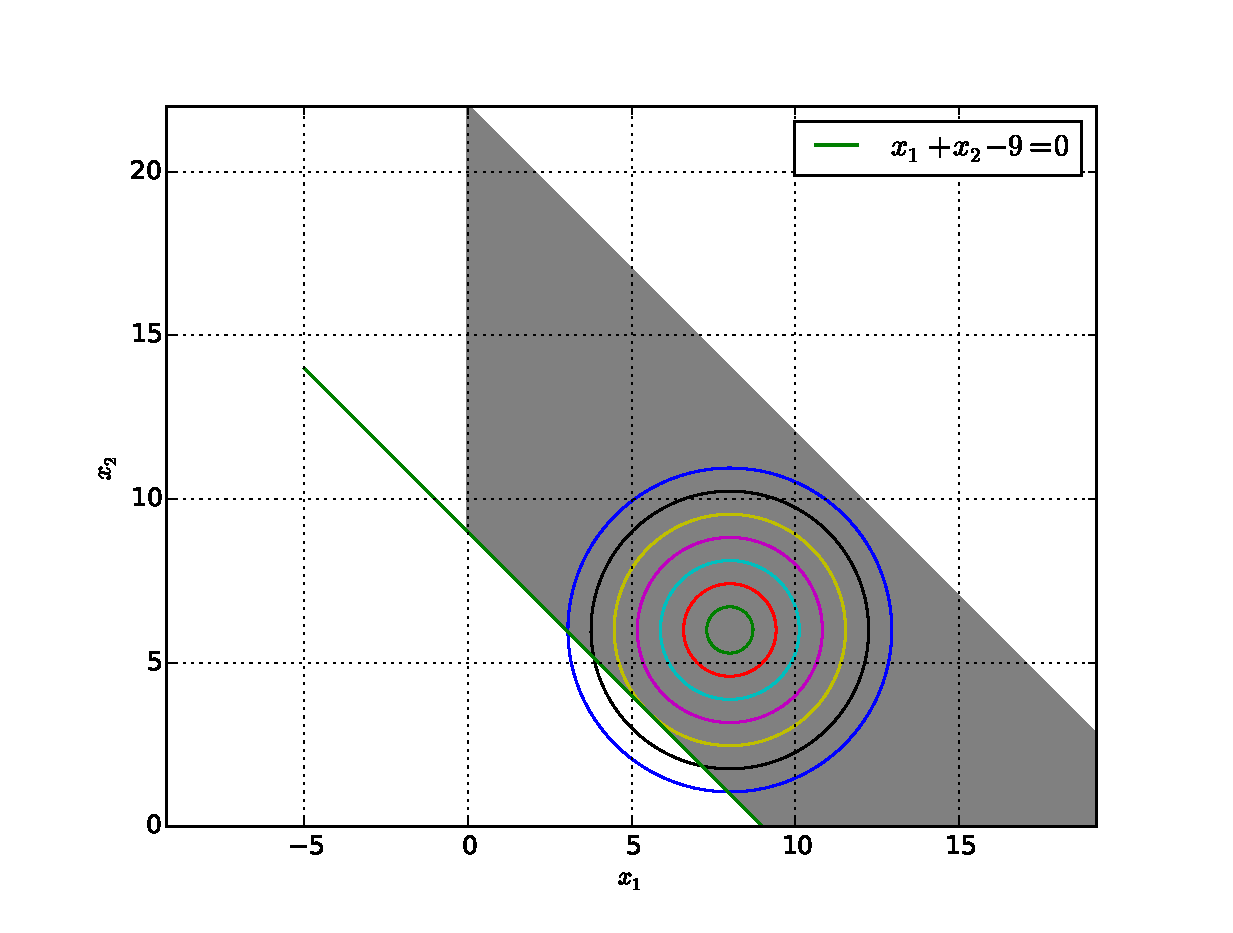
\includegraphics[width=\columnwidth]{./figs/2.4.eps}
%\caption{ Smallest circle in the shaded region is a point.}
%\label{fig.2.4}	
%\end{figure}
%
\item
\label{ch2_lagrange_fail}
Now use the method of Lagrange multipliers to solve  problem \ref{ch2_constraint} and compare with the graphical solution.  Comment.

%
\solution Using the method of Lagrange multipliers, the solution is the same as the one obtained in  problem \ref{ch2_constraint}, which is different from the graphical solution.  This means that the Lagrange multipliers method cannot be applied blindly.
\item
Repeat problem \ref{ch2_lagrange_fail} by keeping 
 $\lambda=0$.   Comment.

\solution Keeping $\lambda = 0$ results in $\vec{x}=\myvec{ 8\\ 6}$, which is the correct solution.  The minimum value of $f\brak{\mbf{x}}$ without any constraints lies in the region $g\brak{\mbf{x}} = 0$.  In this case, $\lambda = 0$.  
%
%
\item
\label{ch2_constraint_border}
Find a graphical solution for minimising
\begin{align}
f\brak{\mbf{x}}
% = (x_1-8)^2 + (x_2-6)^2
\end{align}
with constraint
\begin{align}
%\label{convex-constraint}
g\brak{\mbf{x}} \leq 0
%= x_1 + x_2 - 9 .
\end{align}
Summarize your observations.

%
\solution In Fig. \ref{fig.2.7}, the shaded region represents the constraint.  Thus, the solution is the same as the one in problem \ref{ch2_constraint}. This implies that the method of
Lagrange multipliers can be used to solve the optimization problem with this inequality constraint as well.  Table \ref{table.2.7} summarizes the conditions for this based on the observations so far.
\begin{lstlisting}
wget https://raw.githubusercontent.com/gadepall/optimization/master/manual/codes/2.7.py
\end{lstlisting}

%
%\begin{figure}[!ht]
%\centering
%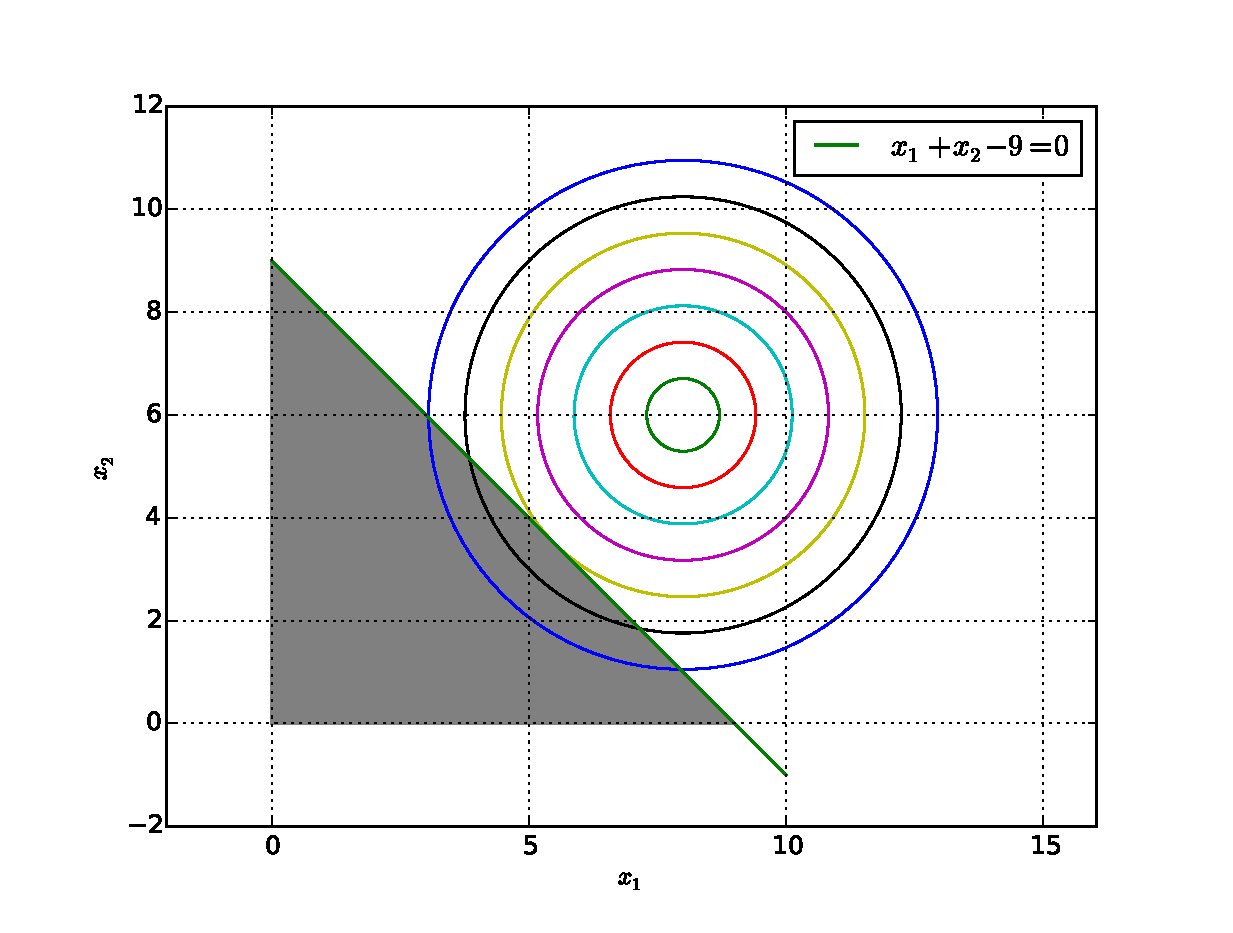
\includegraphics[width=\columnwidth]{./figs/2.7.eps}
%\caption{ Finding $ \displaystyle \min_{\mbf{x}}f\brak{\mbf{x}}$.}
%\label{fig.2.7}	
%\end{figure}
%%%%%%%%%%%%%%%%%%%%%%%%%%%%%%%%%%%%%%%%%%%%%%%%%%%%%%%%%%%%%%%%%%%%%%%
%%                                                                  %%
%%  This is the header of a LaTeX2e file exported from Gnumeric.    %%
%%                                                                  %%
%%  This file can be compiled as it stands or included in another   %%
%%  LaTeX document. The table is based on the longtable package so  %%
%%  the longtable options (headers, footers...) can be set in the   %%
%%  preamble section below (see PRAMBLE).                           %%
%%                                                                  %%
%%  To include the file in another, the following two lines must be %%
%%  in the including file:                                          %%
%%        \def\inputGnumericTable{}                                 %%
%%  at the beginning of the file and:                               %%
%%        \input{name-of-this-file.tex}                             %%
%%  where the table is to be placed. Note also that the including   %%
%%  file must use the following packages for the table to be        %%
%%  rendered correctly:                                             %%
%%    \usepackage[latin1]{inputenc}                                 %%
%%    \usepackage{color}                                            %%
%%    \usepackage{array}                                            %%
%%    \usepackage{longtable}                                        %%
%%    \usepackage{calc}                                             %%
%%    \usepackage{multirow}                                         %%
%%    \usepackage{hhline}                                           %%
%%    \usepackage{ifthen}                                           %%
%%  optionally (for landscape tables embedded in another document): %%
%%    \usepackage{lscape}                                           %%
%%                                                                  %%
%%%%%%%%%%%%%%%%%%%%%%%%%%%%%%%%%%%%%%%%%%%%%%%%%%%%%%%%%%%%%%%%%%%%%%



%%  This section checks if we are begin input into another file or  %%
%%  the file will be compiled alone. First use a macro taken from   %%
%%  the TeXbook ex 7.7 (suggestion of Han-Wen Nienhuys).            %%
\def\ifundefined#1{\expandafter\ifx\csname#1\endcsname\relax}


%%  Check for the \def token for inputed files. If it is not        %%
%%  defined, the file will be processed as a standalone and the     %%
%%  preamble will be used.                                          %%
\ifundefined{inputGnumericTable}

%%  We must be able to close or not the document at the end.        %%
	\def\gnumericTableEnd{\end{document}}


%%%%%%%%%%%%%%%%%%%%%%%%%%%%%%%%%%%%%%%%%%%%%%%%%%%%%%%%%%%%%%%%%%%%%%
%%                                                                  %%
%%  This is the PREAMBLE. Change these values to get the right      %%
%%  paper size and other niceties.                                  %%
%%                                                                  %%
%%%%%%%%%%%%%%%%%%%%%%%%%%%%%%%%%%%%%%%%%%%%%%%%%%%%%%%%%%%%%%%%%%%%%%

	\documentclass[12pt%
			  %,landscape%
                    ]{report}
       \usepackage[latin1]{inputenc}
       \usepackage{fullpage}
       \usepackage{color}
       \usepackage{array}
       \usepackage{longtable}
       \usepackage{calc}
       \usepackage{multirow}
       \usepackage{hhline}
       \usepackage{ifthen}

	\begin{document}


%%  End of the preamble for the standalone. The next section is for %%
%%  documents which are included into other LaTeX2e files.          %%
\else

%%  We are not a stand alone document. For a regular table, we will %%
%%  have no preamble and only define the closing to mean nothing.   %%
    \def\gnumericTableEnd{}

%%  If we want landscape mode in an embedded document, comment out  %%
%%  the line above and uncomment the two below. The table will      %%
%%  begin on a new page and run in landscape mode.                  %%
%       \def\gnumericTableEnd{\end{landscape}}
%       \begin{landscape}


%%  End of the else clause for this file being \input.              %%
\fi

%%%%%%%%%%%%%%%%%%%%%%%%%%%%%%%%%%%%%%%%%%%%%%%%%%%%%%%%%%%%%%%%%%%%%%
%%                                                                  %%
%%  The rest is the gnumeric table, except for the closing          %%
%%  statement. Changes below will alter the table's appearance.     %%
%%                                                                  %%
%%%%%%%%%%%%%%%%%%%%%%%%%%%%%%%%%%%%%%%%%%%%%%%%%%%%%%%%%%%%%%%%%%%%%%

\providecommand{\gnumericmathit}[1]{#1} 
%%  Uncomment the next line if you would like your numbers to be in %%
%%  italics if they are italizised in the gnumeric table.           %%
%\renewcommand{\gnumericmathit}[1]{\mathit{#1}}
\providecommand{\gnumericPB}[1]%
{\let\gnumericTemp=\\#1\let\\=\gnumericTemp\hspace{0pt}}
 \ifundefined{gnumericTableWidthDefined}
        \newlength{\gnumericTableWidth}
        \newlength{\gnumericTableWidthComplete}
        \newlength{\gnumericMultiRowLength}
        \global\def\gnumericTableWidthDefined{}
 \fi
%% The following setting protects this code from babel shorthands.  %%
 \ifthenelse{\isundefined{\languageshorthands}}{}{\languageshorthands{english}}
%%  The default table format retains the relative column widths of  %%
%%  gnumeric. They can easily be changed to c, r or l. In that case %%
%%  you may want to comment out the next line and uncomment the one %%
%%  thereafter                                                      %%
\providecommand\gnumbox{\makebox[0pt]}
%%\providecommand\gnumbox[1][]{\makebox}

%% to adjust positions in multirow situations                       %%
\setlength{\bigstrutjot}{\jot}
\setlength{\extrarowheight}{\doublerulesep}

%%  The \setlongtables command keeps column widths the same across  %%
%%  pages. Simply comment out next line for varying column widths.  %%
\setlongtables

\setlength\gnumericTableWidth{%
	53pt+%
	58pt+%
	55pt+%
0pt}
\def\gumericNumCols{3}
\setlength\gnumericTableWidthComplete{\gnumericTableWidth+%
         \tabcolsep*\gumericNumCols*2+\arrayrulewidth*\gumericNumCols}
\ifthenelse{\lengthtest{\gnumericTableWidthComplete > \linewidth}}%
         {\def\gnumericScale{\ratio{\linewidth-%
                        \tabcolsep*\gumericNumCols*2-%
                        \arrayrulewidth*\gumericNumCols}%
{\gnumericTableWidth}}}%
{\def\gnumericScale{1}}

%%%%%%%%%%%%%%%%%%%%%%%%%%%%%%%%%%%%%%%%%%%%%%%%%%%%%%%%%%%%%%%%%%%%%%
%%                                                                  %%
%% The following are the widths of the various columns. We are      %%
%% defining them here because then they are easier to change.       %%
%% Depending on the cell formats we may use them more than once.    %%
%%                                                                  %%
%%%%%%%%%%%%%%%%%%%%%%%%%%%%%%%%%%%%%%%%%%%%%%%%%%%%%%%%%%%%%%%%%%%%%%

\ifthenelse{\isundefined{\gnumericColA}}{\newlength{\gnumericColA}}{}\settowidth{\gnumericColA}{\begin{tabular}{@{}p{53pt*\gnumericScale}@{}}x\end{tabular}}
\ifthenelse{\isundefined{\gnumericColB}}{\newlength{\gnumericColB}}{}\settowidth{\gnumericColB}{\begin{tabular}{@{}p{58pt*\gnumericScale}@{}}x\end{tabular}}
\ifthenelse{\isundefined{\gnumericColC}}{\newlength{\gnumericColC}}{}\settowidth{\gnumericColC}{\begin{tabular}{@{}p{55pt*\gnumericScale}@{}}x\end{tabular}}

\begin{tabular}[c]{%
	b{\gnumericColA}%
	b{\gnumericColB}%
	b{\gnumericColC}%
	}

%%%%%%%%%%%%%%%%%%%%%%%%%%%%%%%%%%%%%%%%%%%%%%%%%%%%%%%%%%%%%%%%%%%%%%
%%  The longtable options. (Caption, headers... see Goosens, p.124) %%            \\	%
 %\hline	% Across the top of the table.
%%  The rest of these options are table rows which are placed on    %%
%%  the first, last or every page. Use \multicolumn if you want.    %%

%%  Header for the first page.                                      %%
%	\multicolumn{3}{c}{The First Header} \\ \hline 
%	\multicolumn{1}{c}{colTag}	%Column 1
%	&\multicolumn{1}{c}{colTag}	%Column 2
%	&\multicolumn{1}{c}{colTag}	\\ \hline %Last column
%	\endfirsthead

%%  The running header definition.                                  %%
%	\hline
%	\multicolumn{3}{l}{\ldots\small\slshape continued} \\ \hline
%	\multicolumn{1}{c}{colTag}	%Column 1
%	&\multicolumn{1}{c}{colTag}	%Column 2
%	&\multicolumn{1}{c}{colTag}	\\ \hline %Last column
%	\endhead

%%  The running footer definition.                                  %%
%	\hline
%	\multicolumn{3}{r}{\small\slshape continued\ldots} \\
%	\endfoot

%%  The ending footer definition.                                   %%
%	\multicolumn{3}{c}{That's all folks} \\ \hline 
%	\endlastfoot
%%%%%%%%%%%%%%%%%%%%%%%%%%%%%%%%%%%%%%%%%%%%%%%%%%%%%%%%%%%%%%%%%%%%%%

\hhline{|-|-|-}
	 \multicolumn{1}{|p{\gnumericColA}|}%
	{\gnumericPB{\centering}\textbf{Cost}}
	&\multicolumn{1}{p{\gnumericColB}|}%
	{\gnumericPB{\centering}\textbf{Constraint}}
	&\multicolumn{1}{p{\gnumericColC}|}%
	{\gnumericPB{\centering}\textbf{$\lambda$}}
\\
\hhline{|---|}
	 \multicolumn{1}{|p{\gnumericColA}|}%
	{\setlength{\gnumericMultiRowLength}{0pt}%
	 \addtolength{\gnumericMultiRowLength}{\gnumericColA}%
	 \multirow{3}[1]{\gnumericMultiRowLength}{\parbox{\gnumericMultiRowLength}{%
	 \gnumericPB{\centering}$f\brak{\mbf{x}}$}}}
	&\multicolumn{1}{p{\gnumericColB}|}%
	{\gnumericPB{\centering}$g\brak{\mbf{x}} = 0$}
	&\multicolumn{1}{p{\gnumericColC}|}%
	{\gnumericPB{\centering} $<$ 0}
\\
\hhline{~|--|}
	 \multicolumn{1}{|p{\gnumericColA}|}%
	{}
	&\multicolumn{1}{p{\gnumericColB}|}%
	{\gnumericPB{\centering}$g\brak{\mbf{x}} \geq 0 $}
	&\multicolumn{1}{p{\gnumericColC}|}%
	{\gnumericPB{\centering}0}
\\
\hhline{~|--|}
	 \multicolumn{1}{|p{\gnumericColA}|}%
	{}
	&\multicolumn{1}{p{\gnumericColB}|}%
	{\gnumericPB{\centering}$g\brak{\mbf{x}}\leq 0 $}
	&\multicolumn{1}{p{\gnumericColC}|}%
	{\gnumericPB{\centering} $<$ 0}
\\
\hhline{|-|-|-|}
\end{tabular}

\ifthenelse{\isundefined{\languageshorthands}}{}{\languageshorthands{\languagename}}
\gnumericTableEnd

%
\item
\label{ch2_prob_upper}
Find a graphical solution for 	 
	 \begin{align}
	 \label{ch2_second_min}
	\min_{\mbf{x}} f\brak{\mbf{x}} = \norm{\vec{x}-\myvec{8\\6}}^2
	 \end{align}
	 with constraint
	 \begin{align}
	 \label{ch2_second_const}
	 g\brak{\mbf{x}} = \myvec{1 & 1}\vec{x} - 18 = 0
	 \end{align}
	 
%
\solution
%	
\begin{lstlisting}
wget https://raw.githubusercontent.com/gadepall/optimization/master/manual/codes/2.8.py
\end{lstlisting}

%
%\begin{figure}[!ht]
%\centering
%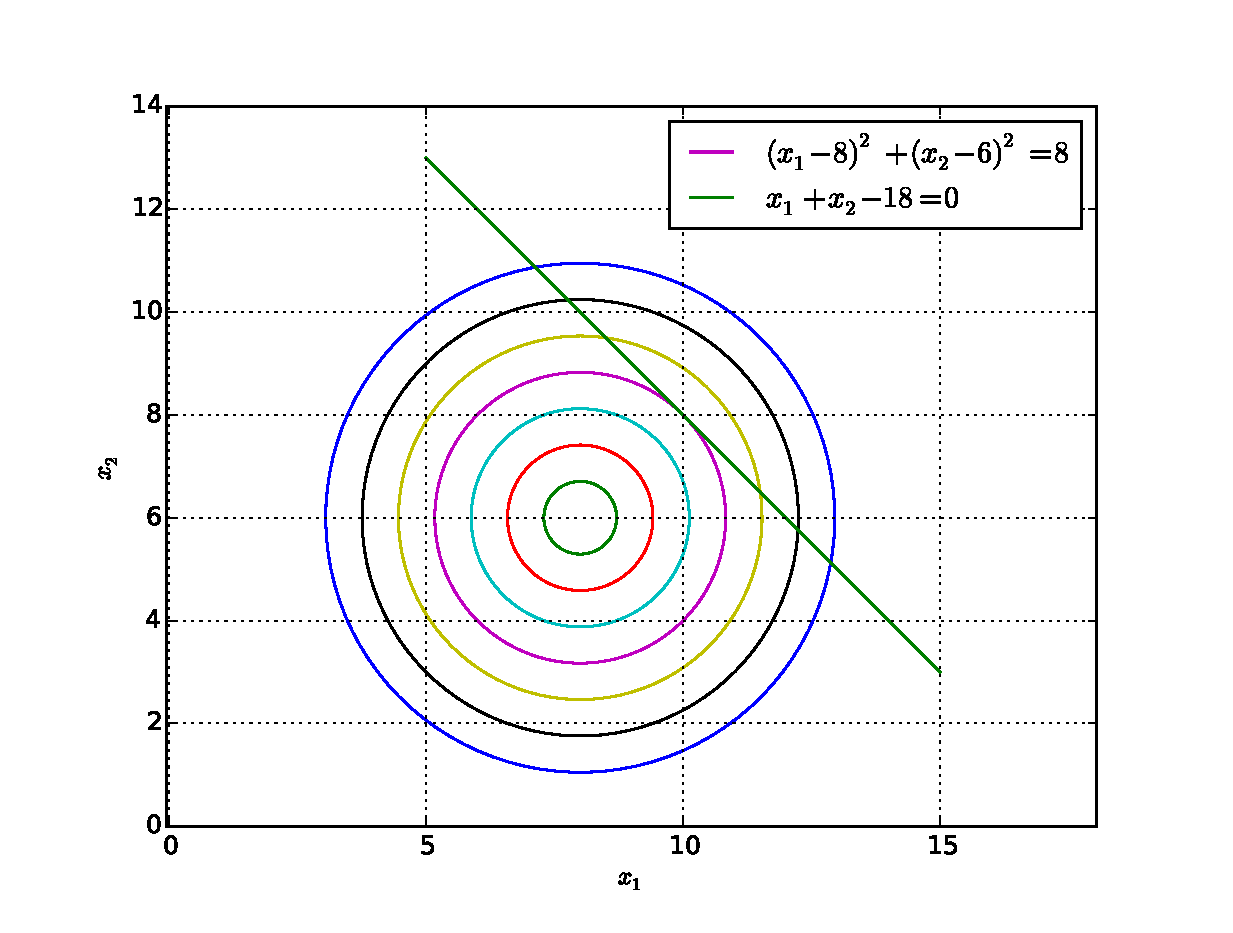
\includegraphics[width=\columnwidth]{./figs/2.8.eps}
%\caption{ Finding $ \displaystyle \min_{\mbf{x}}f\brak{\mbf{x}}$.}
%\label{fig.2.8}	
%\end{figure}
%
\item
Repeat problem \ref{ch2_prob_upper} using the method of Lagrange mutipliers.  What is the sign of $\lambda$?

%
\solution
%From \eqref{ch2_second_min} and \eqref{ch2_second_const}, 
%%
%\begin{align}
%L\brak{\mbf{x},\lambda} &= (x_1-8)^2 + (x_2-6)^2 - \lambda \brak{x_1 + x_2 - 18} \\
%\Rightarrow \nabla L\brak{\mbf{x},\lambda}  & = 
%\begin{pmatrix}
%2x_1  - 16 - \lambda \\
%2x_2 - 12 - \lambda \\
%x_1 + x_2 -18
%\end{pmatrix}
%\\
%&=
%\begin{pmatrix}
%2 &0 & - 1 \\
%0 &2 & - 1 \\
%1 & 1 & 0 
%\end{pmatrix}
%\begin{pmatrix}
%x_1 \\
%x_2 \\
%\lambda
%\end{pmatrix}
%= 
%\begin{pmatrix}
%16 \\
% 12 \\
%18
%\end{pmatrix}
%=
%0 
%\\
%\Rightarrow 
%\begin{pmatrix}
%x_1 \\
%x_2 \\
%\lambda
%\end{pmatrix}
%&= 
%\begin{pmatrix}
%10 \\
% 8 \\
%4
%\end{pmatrix}
%\end{align}
%%
Using the following python script, $\lambda$ is positive and the minimum value of $f$ is 8.
%	
\begin{lstlisting}
wget https://raw.githubusercontent.com/gadepall/optimization/master/manual/codes/2.9.py
\end{lstlisting}

%
%
\item
\label{ch2_prob_upper_cond}
Solve
	 \begin{align}
%	 \label{ch2_second_min}
	\min_{\mbf{x}} f\brak{\mbf{x}} 
%= (x_1-8)^2 + (x_2-6)^2
	 \end{align}
	 with constraint
	 \begin{align}
%	 \label{ch2_second_const}
	 g\brak{\mbf{x}} 
%= x_1 + x_2 - 18 
\geq 0 
	 \end{align}
	 
%
\solution Since the unconstrained solution is outside the region $g\brak{\mbf{x}} \geq 0$, the solution is the same as the one in problem \ref{ch2_prob_upper}.
%
\item
Based on the problems so far, generalise the Lagrange multipliers method for 
%
	 \begin{align}
	 \label{ch2_lagrange_ineq}
	\min_{\mbf{x}} f\brak{\mbf{x}} , \quad 
	 g\brak{\mbf{x}}  \geq 0 
	 \end{align}
%

%
\solution
Considering $L\brak{\mbf{x},\lambda} = f\brak{\mbf{x}} - \lambda g\brak{\mbf{x}}$, for $g\brak{\mbf{x}} = \myvec{1 & 1}\vec{x} - 18 \geq 0$ we found $\lambda > 0 $ and for $g\brak{\mbf{x}} = \myvec{1 & 1}\vec{x} - 9 \leq 0, \lambda < 0$. A single condition can be obtained by framing the optimization problem as
%
	 \begin{align}
	 \label{ch2_lagrange_ineq_summary}
	\min_{\mbf{x}} f\brak{\mbf{x}} , \quad 
	 g\brak{\mbf{x}}  \leq 0 
	 \end{align}
%
with the Lagrangian
%
\begin{equation}
%\label{ch2_kkt_necessary}
L\brak{\mbf{x},\lambda} = f\brak{\mbf{x}} + \lambda g\brak{\mbf{x}}, %\quad  \lambda > 0,  g\brak{\mbf{x}} \leq 0.
\end{equation}
%
provided
%
\begin{equation}
\label{ch2_kkt_necessary}
\nabla L\brak{\mbf{x},\lambda} = 0 \Rightarrow \lambda > 0
\end{equation}
else, $\lambda = 0$.
\end{enumerate}

